\section{SRM Methodology}
\label{sec:2}

The existing methodologies that are most used in the context of solar resources forecasting, to facilitate integration and management of PV plants, smart grid control, or energy trading on the spot market, are based on the time series formalism and numerical weather prediction (NWP). Comparing these two classes of methods, the former is based on extrapolation of data, whereas the latter solves the governing partial differential equations which describes the state of the atmosphere. Since the time series approaches are far less computational demanding than NWP, they are more attractive in terms of forecast benchmarking. In this paper, all benchmarking methods considered are in accordance with time series approaches; they are abbreviated as statistical reference methods (SRMs).

Considering a signal $x$ with samples $x_t$ being regularly-spaced values in time, and transforming it such that $x^c_t\equiv x_t-\mathbb{E}[x]$, which implies the transformed variable has expected value: $\mathbb{E}[x^c]=0$. One fundamental way to describe such a signal is to assume the forecast is a function of the most recent observation(s), or an autoregressive (AR) model. For a forecast at horizon $h$ and a direct multi-step forecast strategy\footnote{to contrast with recursive multi-step forecast \citep{Bontempi2013} where the prediction for the prior time step is used as an input for making a prediction on the following time step}, it is expressed:

\begin{equation}
\label{eq:eq1}
{x}_{t+h}^c=\alpha x^c_t+\omega_{t+h},
\end{equation}
where $x^c_t$ is a centered time-dependant signal, $\alpha$ ($\vert \alpha \vert<1$ for process stability) is a gain term and $\omega$ is additive noise. The direct strategy could be applied because in solar forecasting context this is often the best method although there is no real consensus on this subject. As mentioned by \citet {Taieb2012RecursiveAD}, ``Choosing between these different strategies involves a trade-off between bias and estimation variance". Under the state space framework in the discrete domain where Kalman filter is often used, $x^c_t$ could be defined as the state vector of the process at time $t$, and $\alpha$ the state transition parameter of the process from the state at $t$ to the state at $t+h$, assuming stationarity over time. $\omega$ is the associated zero-mean white noise process, i.e.\, $\omega\sim \mathcal{N}(0, \sigma^2_{\omega})$ with $\sigma^2_{\omega}=\mathbb{E}[\omega_t^2]$. 

With this in mind, observations on this variable are contained in the series $y_t$. The centered form, denoted $y^c_t$ can be modeled by the observation equation:

\begin{equation}
\label{eq:eq2}
y^c_{t}\equiv y_t-\mathbb{E}(y)=x^c_t+v_{t},
\end{equation}
where $y_t$ is the actual measurement of $x$ at time $t$ and $v_t$ is the associated measurement error with $v\sim\mathcal{N}(0,\sigma^2_{v})$. Note that the hypothesis $\mathbb{E}(x)=\mathbb{E}(y)\equiv \bar{y}$ is implied in Eq.(\ref{eq:eq2}) and therefore, a bias in the measurement would be detrimental: a quality control of the sensors is a prohibitive prerequisite. 

\subsection{Usual Benchmark Methods for Meteorological Time Series}
There are many reference methods in meteorology and mainly in solar radiation. In this section and in \ref{appendix}, we will list the most commonly used ones.  

\subsubsection{Persistence \textnormal{(PER)}}
\label{sec:subsec1}
Persistence is the simplest case where $\alpha=1$ in Eq.(\ref{eq:eq1}), the prediction of $x^c_{t+h}$ denoted $\widehat{x}^c_{t+h}$ becomes:

\begin{equation}
\label{eq:eq3}
\widehat{x}^c_{t+h}=x^c_t
\end{equation}
which implies that $\widehat{x}_{t+h}=y_t$. This model (see \ref{algo:Pers} for details) is very reliable when the  meteorological data series has a very low variability but it quickly becomes ineffective with very noisy, periodic or trending signals. However, in  operational cases (forecasting for energy or power management), when the user needs a forecast and when there is no measurement history, it is often the only way to proceed in the nowcasting case (from 1h to 6h). For benchmarking at larger horizons, a solution (and undoubtedly the best alternative) would be the use of climatology. 

\subsubsection{Climatology \textnormal{(CLIM)}}
\label{sec:subsec2}
If in the previous case the method used was only valid for strongly persistent phenomenona (low variability), the model presented here corresponds to the case where there is no statistical dependence between the different measurements (i.e.\ white noise). In this case, we should choose $\alpha= 0$ where it immediately becomes $\widehat{x}^c_{t+h}=0$ and therefore $\widehat{x}_{t+h}^{\,}=\mathbb{E}(y)$ (historical mean). This model (see \ref{algo:Clim} for details), though simple, should not be overlooked, because as soon as the autocorrelation coefficient $\rho$ comes close to 0, it is often the best way to attain a minimum forecast error. This model becomes interesting when predicting meteorological time series, and when deep horizons close to the predictability limit of chaotic phenomena are studied. 

\subsubsection{\textnormal{AR(1)} or Climatology--Persistence \textnormal{(CLIPER)}}
\label{sec:AR}
In this section the link between the AR(1) estimate and the well-named ``climatology--persistence combination,'' or CLIPER for short, is shown. This kind of model can be considered as a reference because it is easy to implement and does not require any learning phase. Hence, it is easy to use and robust in case of data are suddenly missing due to a detector failure if the forecasts are used automatically in operational mode. Now, consider the Yule--Walker equations \citep{175742} or equivalently multiply Eq.(\ref{eq:eq1}) by $x^c_t$ and take the expectation value. $x^c_t$ is considered as a stationary process in the weak sense in the rest of the paper (also denoted wide-sense stationarity, or covariance stationarity). It follows that:

\begin{equation}
\label{eq:eq4bis}
\mathbb{E}[x^c_{t+h}x^c_{t}]=\mathbb{E}[\alpha x^c_tx^c_t+\omega_{t+h}x^c_t].
\end{equation}

After some mathematical considerations detailed in \ref{appendix:cliper} and using the correlation factor $\rho(h)$, it comes that the prediction can be expressed by:

\begin{equation}
\label{eq:CLIPER}
\widehat{x}_{t+h}=\rho(h)y_t+\left[1-\rho(h)\right]\mathbb{E}(y).
\end{equation}

An alternative, and shorter, way to arrive at Eq.~(\ref{eq:CLIPER}) can be found in \citep{doi:10.1063/1.5114985}, in which the same results can be obtained by minimizing the mean square error (MSE) of CLIPER forecasts. The pseudo-code used to predict with CLIPER is given in \ref{algo:ClimPers}.




\subsubsection{Simple Exponential Smoothing \textnormal{(ES)}}
\label{sec:ETS}
Forecasts are calculated using weights that decrease exponentially as data become older (where $\vert \alpha \vert <1$ is the smoothing parameter) as described in Eq.(\ref{eq:ES}) \citep{hyndman_forecasting_2018}.

\begin{equation}
\label{eq:ES}
    \widehat{x}^c_{t+h}=\alpha x^c_t+\alpha(1-\alpha)x^c_{t-1}+\alpha(1-\alpha)^2x^c_{t-2}+...
\end{equation}
That is, all forecasts take the same value ($h$-step-ahead forecast is constant $\forall h$), equal to the last level component. Remember that these forecasts are only  suitable if the time series has no trend or seasonal component. Applying the same tools exposed in the beginning of Section \ref{sec:2}, Eq.(\ref{eq:ES}) can be replaced with:

\begin{equation}
\label{eq:eq7bis}
    \widehat{x}_{t+h}-\bar{y}=\alpha( y_t-\bar{y})+\alpha(1-\alpha)(y_{t-1}-\bar{y})+\alpha(1-\alpha)^2(y_{t-2}-\bar{y})+...
\end{equation}

The separation of the $\bar{y}$ and $y_{t-i}$ terms leads to:

\begin{equation}
\label{eq:eq7ter}
    \widehat{x}_{t+h}=\bar{y}[1-\alpha-\alpha(1-\alpha)-\alpha(1-\alpha)^2-...] + \alpha y_t+\alpha(1-\alpha)y_{t-1}+\alpha(1-\alpha)^2y_{t-2}+...
\end{equation}

If the second part of this equation (Eq.(\ref{eq:eq7ter})) can be reduced according to the sum $\sum_{i=0}^{n} \alpha(1-\alpha)^i y_{t-i}$, the first term is related to the sum of the first $n+1$ terms of a geometric series (common ratio = $1-\alpha$). In the end, the ES model is given by: 

\begin{equation}
\label{eq:eq7}
    \widehat{x}_{t+h}=\alpha \sum_{i=0}^{n} (1-\alpha)^i y_{t-i} +\bar{y}(1-\alpha)^{n+1},\alpha \neq 0.
\end{equation}

In the exponential smoothing method (see \ref{algo:ES} for details), the predictions lie between the two extremes, the naive persistence $\widehat{x}_{t+h}=y_t$ (when $\alpha=1$) and the simple average $\widehat{x}_{t+h}=\bar{y}$ (when $\alpha=0$), which assumes that all observations are of equal importance, and assigns them equal weights when generating forecasts. In order to be consistent with other methods, we choose to determine $\alpha$ without using an optimization phase. As such, considering that $\alpha=\rho(1)$ we obtain a predictor close to the persistence when $\rho(1)$ is close to 1 and close to the mean when it tends to 0. Note that we could use the relation $ \alpha = \rho (h) $ and this could make sense but we wanted to present the simplest method relating to exponential smoothing.  

\subsection{Proposed Methodologies}
The methods used as reference or so-called naive methods in terms of weather forecasting through the time series formalism are often (and this is the entirely the purpose) very easy to implement. Qualifying the following methods as naive may make one smile given the calculations required to develop it. However, they are only ever performed once, then methods are applicable very simply to whatever the studied time series (solar radiation or not).


\subsubsection{\textnormal{Particular AR(2) } \textnormal{(ARTU)}}
\label{sec:method}
In this part, we propose a methodology that improves the performances of the AR(1) model (or CLIPER) previously discussed in Section (\ref{sec:AR}). We show that, even if this is not part of the initial hypotheses [see Eq.(\ref{eq:minus}-\ref{eq:eq8})], this approach is equivalent to an AR(2), with the difference being that the estimation of the coefficients is only based on the autocorrelations generation---since the method is a particular form of AR(2), it is called ARTU, which is pronounced as ``A-R-two.'' Firstly, it is useful to think of another version of Eq.(\ref{eq:eq1}), in which the state estimate is known to be \textit{not} optimal $({x^{c-}_{t+h}})$.

\begin{equation}
\label{eq:minus}
{x^{c-}_{t+h}}=\alpha x^c_t+\omega_{t+h}.
\end{equation}

We further assume the need for an update ($\widehat{x}^c_{t+h}$) related to a linear combination between $\widehat{x}^{c-}_{t+h}$ ($=\alpha x^c_t$) and the previous innovation (or residual i.e. $y^c_{t}-\widehat{x}^{c-}_{t}$). Shown in Eq.(\ref{eq:eq8}) is the updated form, whereby the factor $K$ can be treated as a gain, and the combination as a filtering process. 

\begin{equation}
\label{eq:eq8}
\widehat{x}^c_{t+h}=\widehat{x}^{c-}_{t+h}+K(y^c_{t}-\widehat{x}^{c-}_{t}).
\end{equation}

Note that this approach, although it is quite close to what is observed with prediction of a classical ARMA(1,1) model \citep{CHATFIELD1988411} or a Kalman filtering \citep{DEGOOIJER2006443}, is different. In the first case, $\omega_{t+h}$  would be the residual of $\widehat{x}^c_{t}$ and not $\widehat{x}^{c-}_{t}$, moreover $K$ would be multiplied by $(y^c_{t}-\widehat{x^c_{t}})$ in Eq.(\ref{eq:eq8}). The second one would require a modification in Eq.(\ref{eq:eq8}), in that, $K$ would be multiplied by $(y^c_{t+h}-\widehat{x}^{c-}_{t+h})$. The assumptions of stationarity formulated in Section \ref{sec:AR} are maintained. From Eq.(\ref{eq:minus}) and Eq.(\ref{eq:eq8}), the forecast can therefore be put in the following form:

\begin{equation}
\label{eq:eq8bis}
\widehat{x}^c_{t+h}=\alpha x^c_t+K(y^c_t-\alpha x^c_{t-h}).
\end{equation}

The transition between states and measurements is:

\begin{equation}
\label{eq:eq8ter}
\widehat{x}_{t+h}-\bar{y}=\alpha(y_t-\bar{y})+K[y_t-\bar{y}-\alpha(y_{t-h}-\bar{y})], 
\end{equation}

% that is equivalent to:
\begin{equation}
\label{eq:eq8b}
\widehat{x}_{t+h}=(K+\alpha)y_t-(K\alpha)y_{t-h}+(1+K\alpha-K-\alpha)\bar{y}.
\end{equation}
A more practical parameterization can be proposed by letting $P=K\alpha$ and $S=K+\alpha$. This allows us to present $\widehat{x}_{t+h}$ as a convex combination of $y_t$, $y_{t-h}$ and $\mathbb{E}(y)$ from the sum $S$ and the product $P$:

\begin{equation}
\label{eq:eq8c}
\widehat{x}_{t+h}=Sy_t-Py_{t-h}+(1+P-S)\bar{y}.
\end{equation}


Using what has just been presented above and in \ref{proof}, the optimal values of $\alpha$ and $K$ can be determined by minimizing the MSE of ARTU forecasts. Based on the results therein, the optimal $\alpha$ and $K$ can be written in functions of a triplet [$R$, $\rho(h)$,$\rho(2h)$], where $\rho(h)$ and $\rho(2h)$ are two correlation coefficients that have already defined previously, and $R=\sigma^2_{v}/\sigma_x^2$ is linked to the quality of the measurement. The ARTU prediction is described by the pseudo-code in \ref{algo:METH}. There are, nevertheless, some hypotheses that have been formulated, especially concerning the stationarity of the studied time series. Indeed, wide-sense stationary assumption (mean and variance are time-independent and autocovariance and autocovariance can be expressed as functions of the time-lag) is necessary to obtain a closed-form in \ref{eq:eq14} allowing to simply propose $S$ and $P$ in Eq.(\ref{eq:eq8c}). This is important to keep in mind, because if we deviate too much from these conditions (that can be qualified as ideal), there is a good chance that the ARTU approach (prediction with Eq.(\ref{eq:eq8b}) according the $\alpha$ and $K$ parameters obtained solving Eq.(\ref{eq:eq14})) does not give satisfactory results. To arrive at an approximately stationary time series in respect to solar radiation, it is customary to use a clear-sky model \citep{SUN2021110087}, which is often simplified from the Beer—Lambert relationship (See Section \ref{sec:season}). 
We would see that the non-stationary phenomenon appears during the temperature and wind speed studies (in Section \ref{sec:other}) where there is no simple knowledge model, where using a ratio to trend allows us to get closer to the ideal and stationary case. 

We computed $\alpha$ and $K$ for values of $\rho(h)$ and $\rho(2h)$ from $-1$ to $+1$ (with an incremental step of 0.01) and for 4 values of $R$ (0, 0.01, 0.05 and 0.1) solving Eq.(\ref{eq:eq14}). An example is given in Fig.\ref{fig:fig1} and other values are available in \url{https://github.com/cyrilvoyant/ARTU.git} (via Matlab\textsuperscript{\tiny\textregistered} codes). What is important to remember is that once these values are known, the forecasts become relatively simple to implement by knowing the autocorrelations of the series studied. The forecast is direct, fast and does not require modeling or learning. The parameters are obtained by data mining approach and the method can then be qualified as na\"ive although a minimum of historical data is necessary. 

A potential limitation on the use of the ARTU approach can be enacted from Eq.(\ref{eq:eq8}). Indeed, by multiplying by $x^c_{t-h}$ and taking the expectation value, it comes Eq.(\ref{eq:eq17}) where we observe a condition between the two correlations of the model.

\begin{equation}
\label{eq:eq17}
\rho(h)^2-\rho(2h)=0.
\end{equation}

This means that predictions can be efficient for autocorrelation factors (ACF) that satisfy this equation but becomes less reliable as soon as we deviate from this case. Note that $\rho(h)=a^{bh}$ is a solution of this equation ($a,b\in\mathbb{R}$ with $ \textnormal{log}(a)b<1$) with the constrain of  $\lvert\rho(h)\rvert<1$. 

As soon as the ACF deviates from the exponential decay, the results are best with the filtering proposed here while when the decay is respected the filtration is not necessary. This induces $K=0$ and $\alpha=\rho(h)$ and the model becomes equivalent to the classical CLIPER presented in Section \ref{sec:AR}. In summary, the best results are observed without filtration and in the presence of the exponential decay of the ACF, but when this one is not observed, the filtration takes all importance and in theory  improves the predictions.

Before going any further, it is thought essential to clarify and discuss the variable $R$. From its construction, we realize that the variance ratio fluctuates between 0 ($ \sigma_x ^ 2  \gg \sigma^2_{v}$) and 1 ($ \sigma_x ^ 2  \sim \sigma^2_{v}$). Usually, the measuring devices used in meteorology are quite efficient, so we can limit the values of $ R $ between $ 0 $ and 10\% of $ \sigma _x ^ 2 $. According to \citet{vuilleumier2017}, one can logically imagine using an $ R $ between 1\% and 5\% . 

Fig. \ref{fig:fig1} shows as example (for $R=0.05$) the values of $\alpha$ and $K$ obtained with the methodology exposed previously. Four areas are visible concerning $K$, bounded by the line $\rho(h)=0$ and the parabola defined by the equation $\rho(2h)=\rho(h)^2$. Magnification of the area related to positives value of $\rho(h)$ and $\rho(2h)$ is proposed in Fig. \ref{fig:fig2}. Positive values correspond to what is usually observed in solar radiation. All the files used to generate the $ \alpha $ and $ K $ coefficients are available in \url{https://github.com/cyrilvoyant/ARTU.git} ($\mathcal{M}(R)$ matrices and codes). 
For a forecast at the horizon $h$, the procedure is as follows:
\begin{itemize}[label=$\looparrowright$]  
\item Calculate $ \rho (h) $ and $ \rho (2h) $ using in-sampling data;
\item Obtain the $ \alpha $ and of $ K $ values by consulting on Figures \ref {fig:fig1} and \ref {fig:fig2} or generating them more precisely using the code available in \ref{algo:METH} and the matrices ($\mathcal{M}(R)$); 
\item Derive forecast using Eq.(\ref {eq:eq8c}). 
\end{itemize}
In the end, let us suppose that we seek to use the filtration previously stated, for a signal concerning $h = 1$, if one estimates $ \rho (1) = 0.4 $ and $ \rho (2) = 0.3 $; we therefore have $\widehat{x}_{t+1}=S{y}_t-Py_{t-1}+(1+P-S)\bar{y}$, Cf. Eqs.~(\ref{eq:eq8})--(\ref{eq:eq8c}), and so:


 \begin{itemize}[label=$\looparrowright$]  
\item $\widehat{x}_{t+1}=0.33y_t+0.16y_{t-1}+0.51\bar{y}$ for $R=0.01$, $\alpha=0.60$ and $K=-0.27$ hence $S=0.33$ and $P=-0.16$;
\item $\widehat{x}_{t+1}=0.34y_t+0.15y_{t-1}+0.51\bar{y}$ for $R=0.05$, $\alpha=0.59$ and $K=-0.25$ hence $S=0.34$ and $P=-0.15$;
\item $\widehat{x}_{t+1}=0.35y_t+0.13y_{t-1}+0.52\bar{y}$ for $R=0.10$, $\alpha=0.58$ and $K=-0.23$ hence $S=0.35$ and $P=-0.13$.
\end{itemize} 



%\begin{landscape}
\begin{figure}
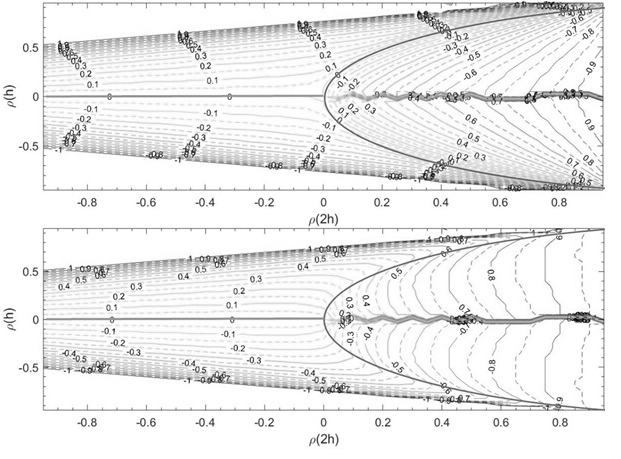
\includegraphics[scale=1.05]{fig1.jpg}% 
\caption{$K$ (top) and $\alpha$ (bottom) values according to the values of $\rho(h)$ and $\rho(2h)$ and for $R^*=0.05$ (resolution of Eq.(\ref{eq:eq14})).} 
\label{fig:fig1} 
\end{figure}
%\end{landscape}

\begin{landscape}
\begin{figure}[tb]
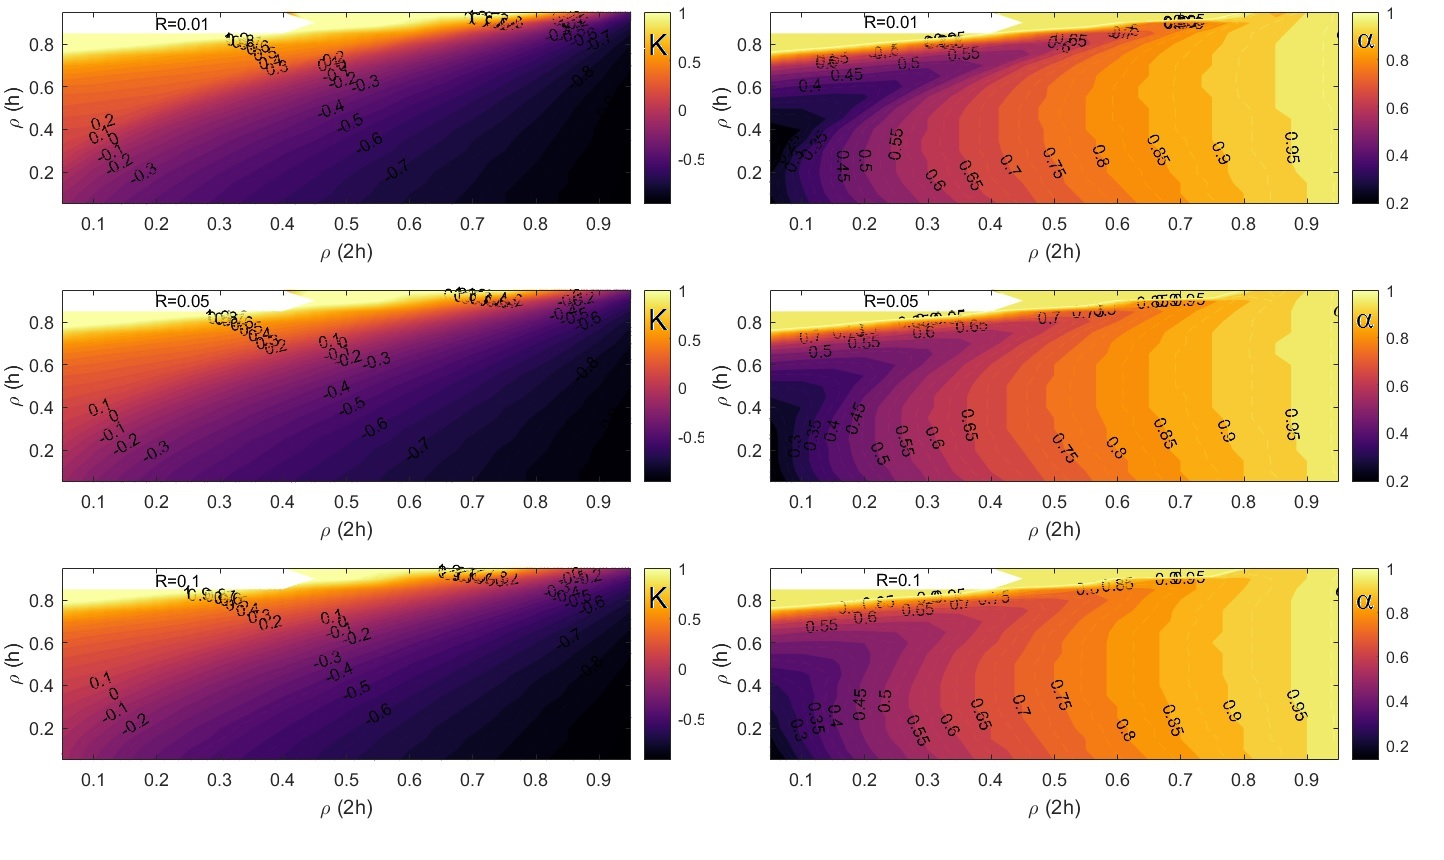
\includegraphics[scale=0.80]{fig2.jpg}% 
\caption{$\alpha$ and $K$ values according to the values of $\rho(h)$, $\rho(2h)$ and $R$} 
\label{fig:fig2}
\end{figure}
\end{landscape}

\subsubsection{The Combination of Methods \textnormal{(COMB)}}
\label{sec:comb}
According to the conclusions related to the M4 forecasting competition \citep{article4}, one of the major findings is related to the combination of methods \citep{SPILIOTIS202159}. In fact, among the most accurate methods, the vast majority (12 of the 17 most accurate) were a combination of statistical approaches. Moreover, this aspect is so important that one innovation was the introduction of a combination reference for benchmarking the accuracy of the methods submitted to the competition. It therefore seems logical to draw inspiration from this remarkable conclusion in order to propose a reference predictive methodology based on the combination of the simple methods presented in this study. Still inspired by \cite{article4} we chose to use the simple arithmetic average of the different outputs of the models although the use of the median may show equally good results in some situations \citep{article5}. %e.g., when the predictive distribution is symmetric.


